% !TeX spellcheck = en_GB
% !TeX encoding = UTF-8

\section{CakeML}
\label{sec:intro:cakeml}

\begin{figure}[t]
  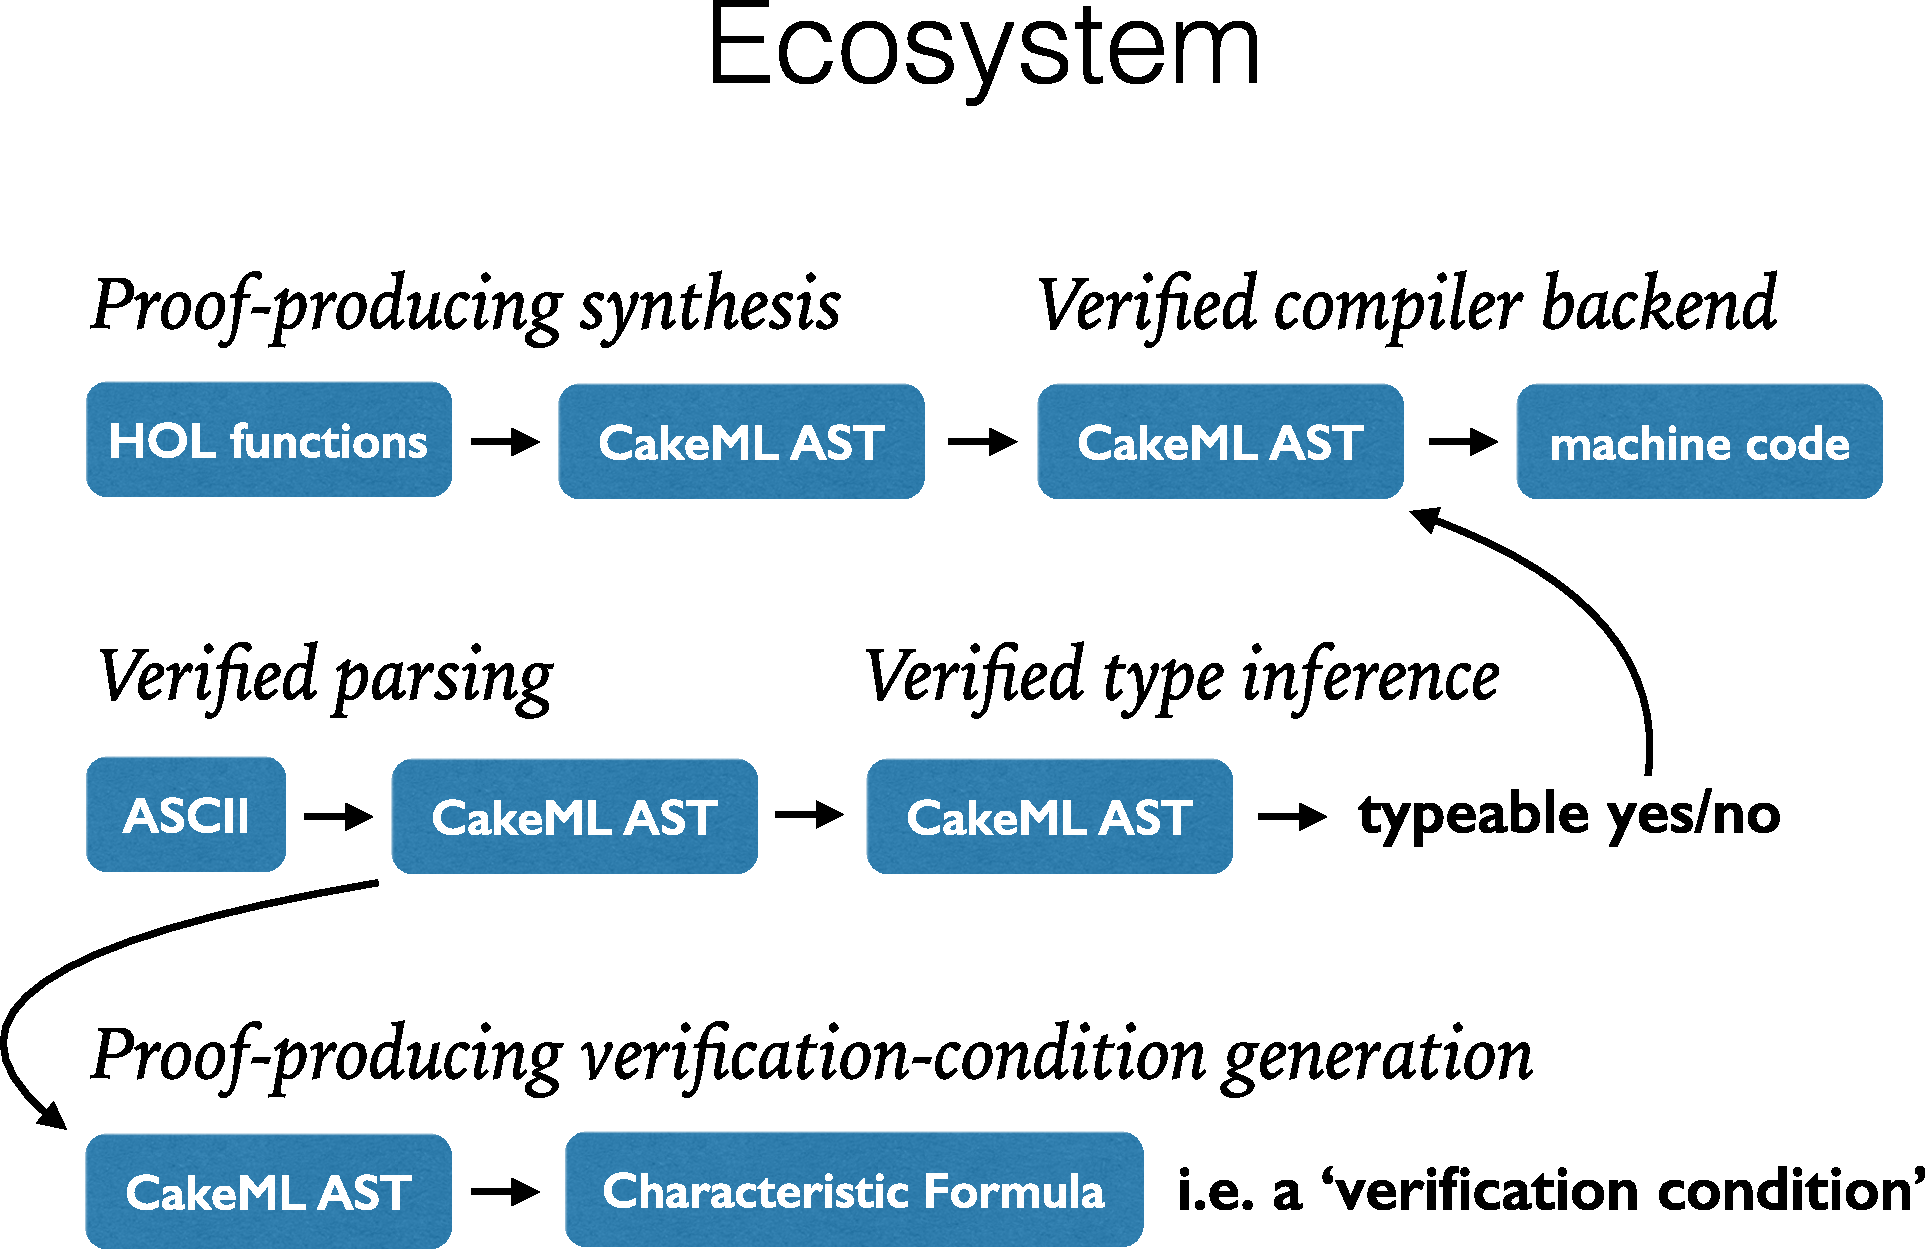
\includegraphics[width=\linewidth]{img/ecosystem.pdf}
  \caption[The CakeML ecosystem]{The CakeML ecosystem\footnotemark}
  \label{fig:intro:cakeml}
\end{figure}
\footnotetext{Image source: \url{https://cakeml.org/ecosystem.png}, used with permission}

\emph{CakeML} is a verified implementation of a subset of Standard ML \cite{kumar2014cakeml,tan2016cakeml}.
To quote the website, it is supplemented by ``an ecosystem of proofs and tools built around the language'' with the ``ecosystem [including] a proven-correct compiler that can bootstrap itself''.\footnote{\url{https://cakeml.org/}}
At time of writing, the project sports over forty developers and contributors.

\cref{fig:intro:cakeml} gives an overview over the ecosystem.
The verified part comprises a parser, type checker, formal semantics and backend for machine code.
The correctness proofs are carried out in the \emph{HOL4} system \cite{hol2014description}.
HOL4 is a proof assistant in the LCF family, similar to Isabelle.

CakeML is an integral part of this work.
My compiler produces CakeML abstract syntax trees and the correctness theorems are justified against its semantics.

\subsection{Semantics}

\begin{code}
  \centering
  \begin{subcode}{.4\linewidth}
    \begin{lstlisting}[language=ML]
type lit =
  | IntLit of integer
  | Char of char
  | StrLit of string
  | Word8 of word8
  | Word64 of word64\end{lstlisting}
  \end{subcode}
  \begin{subcode}{.4\linewidth}
    \begin{lstlisting}
datatype lit =
    IntLit int
  | Char char
  | StrLit string
  | Word8 (8 word)
  | Word64 (64 word)\end{lstlisting}
  \end{subcode}
  \caption{Lem specification of CakeML's type of literals and the resulting Isabelle text}
  \label{code:intro:cakeml:literals}
\end{code}

CakeML's semantics has been specified in \emph{Lem} \cite{mulligan2014lem}, ``a tool for lightweight executable mathematics''.\footnote{\url{https://www.cl.cam.ac.uk/~pes20/lem/}}
It provides a formal specification language that has features comparable to Isabelle/HOL; notably, definition of recursive types, functions and (inductive) predicates.
Lem is capable of compiling these specifications to other specification languages, including Isabelle, HOL4, and Coq.

The remainder of the CakeML ecosystem is implemented in HOL4.
For that, the developers maintain the CakeML semantics in Lem and compile it to HOL4.
Consequently, assuming trust in Lem, the version of the semantics that I use in Isabelle can be considered identical to the one in HOL4.
The Isabelle theories are available in the Archive of Formal Proofs~\cite{hupel2018cakeml}.

The CakeML formalization in Lem consists of multiple parts:
\begin{description}
  \item[Foundation libraries]
    Lem provides a standard library, notably for machine words.
  \item[Abstract syntax]
    As is usual in formalizations of programming languages, datatypes for expressions and values are provided.
  \item[Semantics]
    There are three flavours of semantics: (relational) big step, small step, and functional big step~\cite{owens2016functional}.
    For this thesis, only the big-step semantics is relevant.
\end{description}

\noindent
Note the absence of parsing and printing (i.e., concrete syntax).
This has been developed in HOL4 without the help of Lem, so a translation to Isabelle would be a significant undertaking.

\subsection{Compiler}

The simplest way for a user to interact with CakeML is to write some source code as they would for any other language.
The CakeML project provides a compiler that can be executed on x86-64 systems, producing a binary that may run on a variety of hardware platforms.
That compiler has itself been extracted from a formal specification.
Assuming the correctness of HOL4, every compilation guarantees that the resulting binary works correctly according to the semantics of the source program; in other words, compilation preserves semantics.

Another way to produce a binary program is to use the code extraction facility from HOL4 that goes directly to CakeML abstract syntax trees.
This thesis provides a similar tool, but implemented based on a different approach and for Isabelle/HOL specifications.